\documentclass[10pt]{article}
\usepackage[margin=2.2cm]{geometry}
\usepackage{amsmath,amssymb,booktabs,graphicx,hyperref,natbib}
\title{Adaptive collocation for physics-informed neural networks across P\'eclet numbers:\\
an equal-budget, exact-reference benchmark inside a verified research platform}
\author{Bhavishya}
\date{Research use only. Draft generated from \texttt{results/}; see \texttt{paper/CLAIMS\_AUDIT.md}.}
\begin{document}
\maketitle

\begin{abstract}
% sources: phase3_adaptive_collocation
We test whether residual-based adaptive collocation (RAR, RAD, R3) improves physics-informed neural networks
for transient convection--diffusion as the P\'eclet number grows from 1 to 1000. The reference solution is
exact, the collocation budget and iterations are equal across seven samplers, and the eight seeds are paired.
The PINN error is U-shaped in Pe: median relative $L_2$ errors are 0.1503, 0.0180, 0.0504 and 0.1793 at
Pe = 1, 10, 100 and 1000 with uniform sampling. After Holm correction no adaptive sampler improves on uniform
sampling at Pe $\ge$ 100. At Pe = 1 adaptive samplers are statistically detectably but negligibly worse.
Causal weighting (0.1134) and a hard initial condition (0.0706) reduce the Pe = 1000 error, whereas untuned
Fourier features increase it (0.7894). The Pe = 1 failure is an initial diffusion layer that no sampler
resolves. We report these negative results inside an open platform whose classical solvers are verified,
and we discuss what further work a publishable contribution would require.

\end{abstract}

\section{Introduction}
Physics-informed neural networks promise mesh-free solution of PDEs but are known to struggle with
convection-dominated transport \citep{krishnapriyan2021failure}. Adaptive placement of collocation points is
one of the most frequently proposed remedies \citep{lu2021deepxde,wu2023sampling,daw2022r3}. We ask a narrow,
falsifiable question: \emph{at equal budget, does adaptivity help more as the P\'eclet number grows?} We answer
it for one transient convection--diffusion family with an exact reference, and we report every outcome,
including negative ones. The study is embedded in a research platform (AeroSynapse--Einstein) that provides
verified classical solvers, an independent validation engine and reproducibility tooling.


\section{Literature review}
Physics-informed neural networks (PINNs) minimise a PDE residual evaluated at collocation points
\citep{raissi2017pinn1}. Residual-based adaptive refinement (RAR) adds high-residual points
\citep{lu2021deepxde}; RAD and RAR-D resample from residual-weighted densities and were compared in an
extensive study \citep{wu2023sampling}; R3 retains high-residual points to avoid propagation failures
\citep{daw2022r3}; gradient-aware variants target sharp solutions \citep{zhang2023asm}. Convection-dominated
problems are a documented failure mode of PINNs \citep{krishnapriyan2021failure}, with remedies including
curriculum and sequence-to-sequence training, Lagrangian reformulation \citep{lpinn2022}, causal weighting
\citep{wang2022causal}, adaptive loss weights \citep{wang2021gradient} and loss-weight design for high-P\'eclet
problems \citep{lossweight2025}. Fourier features address spectral bias \citep{tancik2020fourier}. Operator
learning (FNO \citep{li2021fno}, DeepONet \citep{lu2021deeponet}) and deep ensembles
\citep{lakshminarayanan2017ensembles} are used as comparison methods. Public benchmarks include PDEBench
\citep{takamoto2022pdebench}, AirfRANS \citep{bonnet2022airfrans} and The Well \citep{ohana2024well}.

\section{Research gap}
% sources: phase3_adaptive_collocation
Prior comparisons of collocation strategies span many PDEs, budgets and architectures \citep{wu2023sampling,daw2022r3}.
They do not isolate how the benefit of adaptivity depends on the P\'eclet number for a single transient
convection--diffusion family with an \emph{exact} reference, \emph{equal} collocation budgets, paired seeds and
multiple-comparison control. Our gap is therefore narrow and empirical: a controlled measurement, not a new method.


\section{Mathematical formulation}
We study $u_t + u_x = \mathrm{Pe}^{-1}u_{xx}$ on the periodic unit interval for $t\in(0,1]$, with
$u(x,0)=\exp(-(x-x_0)^2/(2\sigma_0^2))$, $x_0=0.25$, $\sigma_0=0.1$. The exact solution follows from the
method of images:
\[ u(x,t)=\sum_{k}\frac{\sigma_0}{\sigma(t)}\exp\!\Big(-\frac{(x-x_0-t-k)^2}{2\sigma(t)^2}\Big),\qquad
\sigma(t)^2=\sigma_0^2+2t/\mathrm{Pe}. \]
Periodicity is enforced exactly by embedding $x\mapsto(\cos2\pi x,\sin2\pi x)$; the initial condition is
a penalty term. The loss is $\mathcal L=\overline{r^2}+\overline{(u(\cdot,0)-u_0)^2}$.

\section{Numerical methods}
The platform's classical solvers (finite differences, finite volumes with upwind/central/QUICK/van Leer
faces, P1 finite elements, a MAC projection Navier--Stokes solver and a Hess--Smith panel method) were
verified by manufactured or analytical solutions (Table~\ref{tab:phase1}) and validated against
\citet{ghia1982} (Table~\ref{tab:phase6_cavity}) and the DFG 2D-1 cylinder benchmark \citep{schafer1996}.
For the PINN study, the reference is exact, so the reference discretisation error is zero (up to image
truncation below $10^{-12}$).
% sources: phase1_verification
\begin{table}[t]\centering\small\caption{Observed order of accuracy (finest pair), Phase 1}\label{tab:phase1}
\begin{tabular}{lll}\toprule
case & finest error & observed order \\ \midrule
heat1d\_cn & 1.48e-05 & 2 \\
heat2d\_cn & 0.000236 & 2 \\
convdiff\_fv\_upwind\_pe50 & 0.007 & 0.955 \\
convdiff\_fv\_central\_pe50 & 4.43e-05 & 2 \\
convdiff\_fv\_quick\_pe50 & 1.22e-05 & 1.99 \\
convdiff\_fv\_vanleer\_pe50 & 2.28e-05 & 2 \\
burgers\_fv & 0.018 & 1.82 \\
wave\_leapfrog & 1.51e-05 & 2 \\
poisson2d\_fd & 0.000683 & 2 \\
poisson2d\_fem\_L2 & 0.000812 & 2 \\
poisson2d\_fem\_H1 & 0.128 & 0.999 \\
poisson1d\_DD & 1.06e-05 & 2 \\
poisson1d\_NR & 0.0001 & 2 \\
poisson1d\_RD & 5.28e-05 & 2 \\
poisson1d\_PP & 0.000201 & 2 \\
\bottomrule\end{tabular}\end{table}

% sources: phase6_fluids_aero
\begin{table}[t]\centering\small\caption{Lid-driven cavity vs Ghia et al. (1982): centre-line RMS differences}\label{tab:phase6\_cavity}
\begin{tabular}{llll}\toprule
case & RMS u & RMS v & converged \\ \midrule
re100\_n32 & 0.0013 & 0.00358 & True \\
re100\_n64 & 0.0018 & 0.00434 & True \\
re400\_n32 & 0.015 & 0.020 & True \\
re400\_n64 & 0.00358 & 0.00444 & True \\
\bottomrule\end{tabular}\end{table}


\section{ML architecture}
MLP, 3 hidden layers of width 32, $\tanh$, Xavier initialisation, Adam ($10^{-3}$, decay 0.9 per 1000
iterations), float32, 4000 iterations, 2000 collocation points, resampling every 250 iterations.

\section{Experimental design}
% sources: phase3_adaptive_collocation
P\'eclet numbers $\{1,10,100,1000\}$; samplers: fixed uniform, uniform resampling, Latin hypercube, scrambled Sobol,
RAR, RAD and R3, all with the same number of collocation points and iterations. Each sampler/P\'eclet cell uses
8 seeds; a seed fixes the network initialisation, so comparisons are paired. The primary metric is the relative
$L_2$ error on a $201\times201$ space--time grid against the exact solution. Tests: two-sided exact Wilcoxon
signed-rank versus uniform, Holm-corrected within each P\'eclet number; Friedman across samplers; percentile
bootstrap 95\% intervals of the median. The hypotheses were written into the experiment record before execution.
Ablations: Fourier features, causal weighting and hard initial conditions.


\section{Baselines}
Uniform random collocation (fixed), uniform resampling, Latin hypercube and scrambled Sobol sequences are the
non-adaptive baselines; Phase 2 adds a supervised network with exact labels and the classical solvers
(Table~\ref{tab:phase2}).
% sources: phase2_pinn_benchmarks
\begin{table}[t]\centering\small\caption{PINN and supervised-baseline relative L2 error vs exact solutions}\label{tab:phase2}
\begin{tabular}{llll}\toprule
case/hard BC & mean & sd & seeds \\ \midrule
heat1d/False & 0.000822 & 9.56e-05 & 3 \\
heat1d/True & 0.000316 & 0.000115 & 3 \\
poisson2d/False & 0.203 & 0.028 & 3 \\
poisson2d/True & 0.018 & 0.00162 & 3 \\
burgers1d/False & 0.020 & 0.014 & 3 \\
convdiff\_pe2/False & 0.332 & 0.00385 & 3 \\
convdiff\_pe10/False & 0.158 & 0.056 & 3 \\
bl\_pe20/False & 0.497 & 0.848 & 3 \\
bl\_pe20/True & 0.000614 & 0.000165 & 3 \\
disk/False & 0.00226 & 0.000146 & 3 \\
disk/True & 0.000405 & 0.000222 & 3 \\
poisson2d/False/annealing & 0.973 & 0.024 & 3 \\
supervised/heat1d & 0.00382 & 0.0019 & 3 \\
supervised/poisson2d & 0.026 & 0.013 & 3 \\
supervised/burgers1d & 0.012 & 0.00141 & 3 \\
supervised/convdiff\_pe10 & 0.068 & 0.022 & 3 \\
\bottomrule\end{tabular}\end{table}


\section{Results}
% sources: phase3_adaptive_collocation
Table~\ref{tab:phase3} lists every cell. With uniform sampling the median relative $L_2$ error is 0.1503 at
Pe = 1, 0.0180 at Pe = 10, 0.0504 at Pe = 100 and 0.1793 at Pe = 1000. At Pe = 1000 the medians range from 0.1658
(R3) to 0.1888 (RAD), and the Friedman test does not reject equality ($p = 0.5461$). At Pe = 100 the smallest
Holm-adjusted $p$ against uniform is 0.3281 (RAD). At Pe = 1, RAR, RAD and R3 are significantly worse
(Holm $p = 0.0469$), with median $\log_{10}$ error ratios of 0.002 to 0.004.

% sources: phase3_adaptive_collocation
\begin{table}[t]\centering\small\caption{Equal-budget sampler comparison (8 seeds; paired Wilcoxon vs uniform, Holm within Pe)}\label{tab:phase3}
\begin{tabular}{lllllll}\toprule
Pe & sampler & median rel. L2 & 95% CI & p (Holm) & significant & wall s \\ \midrule
1.0 & uniform & 0.150 & [0.150, 0.151] & - & - & 39.8 \\
1.0 & uniform\_resample & 0.150 & [0.150, 0.151] & 0.938 & no & 38.4 \\
1.0 & lhs & 0.150 & [0.150, 0.150] & 0.938 & no & 38.6 \\
1.0 & sobol & 0.150 & [0.150, 0.151] & 0.938 & no & 56 \\
1.0 & rar & 0.151 & [0.151, 0.151] & 0.047 & yes & 42.4 \\
1.0 & rad & 0.151 & [0.151, 0.151] & 0.047 & yes & 41.2 \\
1.0 & r3 & 0.152 & [0.151, 0.152] & 0.047 & yes & 42.9 \\
10.0 & uniform & 0.018 & [0.010, 0.037] & - & - & 40.3 \\
10.0 & uniform\_resample & 0.015 & [0.014, 0.036] & 1 & no & 38.8 \\
10.0 & lhs & 0.016 & [0.012, 0.040] & 1 & no & 57.3 \\
10.0 & sobol & 0.014 & [0.011, 0.039] & 1 & no & 44.7 \\
10.0 & rar & 0.025 & [0.018, 0.051] & 0.094 & no & 48.7 \\
10.0 & rad & 0.020 & [0.015, 0.048] & 0.094 & no & 43.7 \\
10.0 & r3 & 0.018 & [0.014, 0.050] & 1 & no & 38.9 \\
100.0 & uniform & 0.050 & [0.033, 0.101] & - & - & 40.3 \\
100.0 & uniform\_resample & 0.050 & [0.038, 0.106] & 1 & no & 40.4 \\
100.0 & lhs & 0.042 & [0.034, 0.113] & 1 & no & 41.7 \\
100.0 & sobol & 0.044 & [0.033, 0.116] & 1 & no & 45.2 \\
100.0 & rar & 0.060 & [0.041, 0.111] & 0.547 & no & 48.1 \\
100.0 & rad & 0.058 & [0.037, 0.113] & 0.328 & no & 67.6 \\
100.0 & r3 & 0.051 & [0.039, 0.102] & 0.594 & no & 87.4 \\
1000.0 & uniform & 0.179 & [0.131, 0.282] & - & - & 90 \\
1000.0 & uniform\_resample & 0.166 & [0.131, 0.298] & 1 & no & 94.1 \\
1000.0 & lhs & 0.167 & [0.112, 0.280] & 1 & no & 127 \\
1000.0 & sobol & 0.182 & [0.116, 0.290] & 1 & no & 122 \\
1000.0 & rar & 0.170 & [0.129, 0.278] & 1 & no & 118 \\
1000.0 & rad & 0.189 & [0.124, 0.306] & 0.234 & no & 126 \\
1000.0 & r3 & 0.166 & [0.116, 0.279] & 1 & no & 111 \\
\bottomrule\end{tabular}\end{table}

\begin{figure}[t]\centering
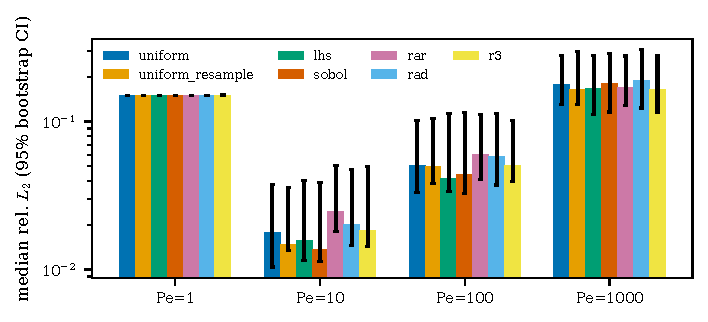
\includegraphics[width=\linewidth]{figures/fig_phase3_samplers.pdf}
\caption{Median relative $L_2$ error with 95\% bootstrap intervals per sampler and P\'eclet number.}
\end{figure}
\begin{figure}[t]\centering
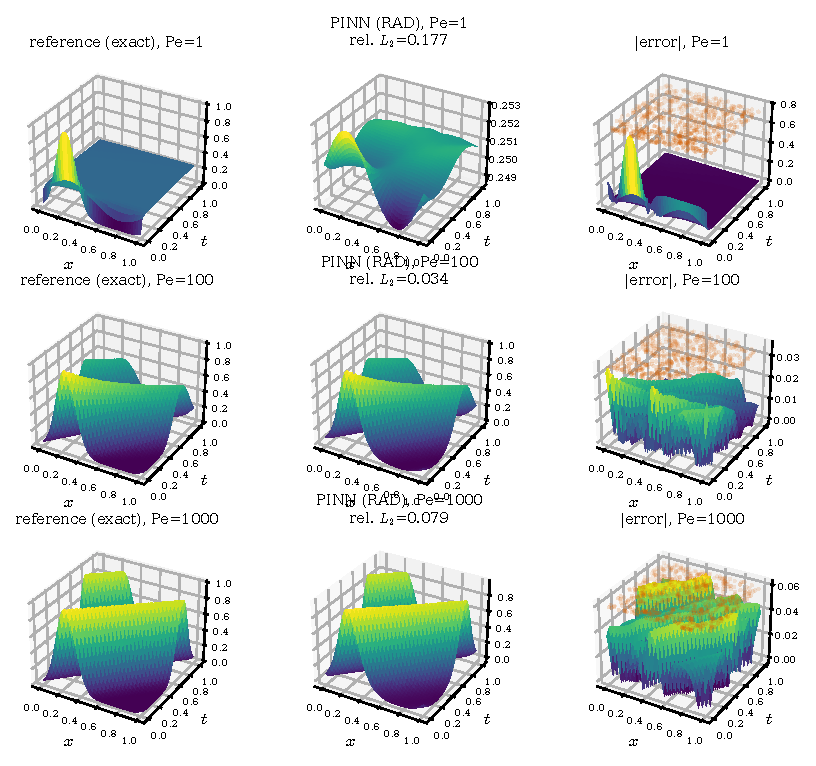
\includegraphics[width=\linewidth]{figures/fig_c_spacetime_surfaces.pdf}
\caption{Space--time solutions: exact reference, PINN (RAD) and absolute error with final collocation points.}
\end{figure}
\begin{figure}[t]\centering
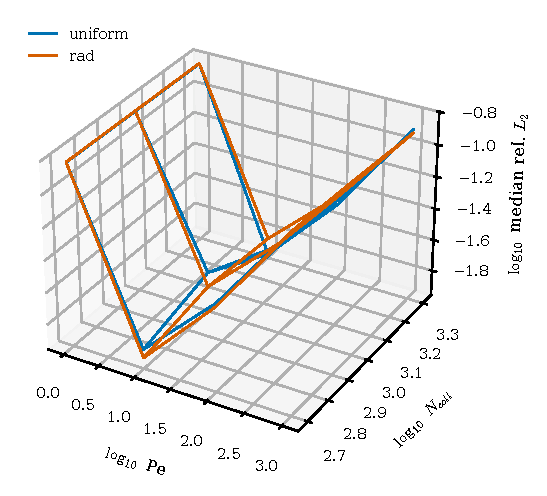
\includegraphics[width=0.6\linewidth]{figures/fig_d_performance_surface.pdf}
\caption{Median error as a function of P\'eclet number, collocation budget and sampler.}
\end{figure}

\section{Error analysis}
% sources: phase3_adaptive_collocation
Errors are dominated by optimisation and approximation, not by the reference (exact). At Pe = 1 all seeds and
samplers land between 0.1500 and 0.1516, and the early-time ($t\le0.05$) median error is 0.5384, against 0.0
reference error: the network systematically misses the initial diffusion layer. At Pe = 1000 the
seed-to-seed spread is large (95\% interval of the uniform median 0.1308 to 0.2825), which indicates
sensitivity to initialisation rather than to point placement.


\section{Ablation studies}
% sources: phase3_adaptive_collocation
\begin{table}[t]\centering\small\caption{Ablations (paired vs the same sampler without the component)}\label{tab:phase3\_ablation}
\begin{tabular}{llllll}\toprule
ablation/Pe/sampler & median & baseline median & p & early-t median & baseline early-t \\ \midrule
causal/1.0/uniform & 0.150 & 0.150 & 0.00781 & 0.536 & 0.538 \\
causal/1000.0/uniform & 0.113 & 0.179 & 0.00781 & 0.087 & 0.133 \\
fourier/1000.0/rad & 0.791 & 0.189 & 0.00781 & 0.793 & 0.153 \\
fourier/1000.0/uniform & 0.789 & 0.179 & 0.00781 & 0.779 & 0.133 \\
hard\_ic/1.0/uniform & 0.239 & 0.150 & 0.023 & 0.270 & 0.538 \\
hard\_ic/1000.0/uniform & 0.071 & 0.179 & 0.016 & 0.011 & 0.133 \\
\bottomrule\end{tabular}\end{table}

% sources: phase3_adaptive_collocation
Holm-corrected over the six ablations (post-hoc), every effect is detectable at the 0.0469 level, the smallest
value attainable with eight paired seeds. Causal weighting lowers the Pe = 1000 median from 0.1793 to 0.1134 but
leaves the Pe = 1 early-time error unchanged (0.5359 vs 0.5384). A hard initial condition lowers the Pe = 1000
median to 0.0706 and halves the early-time error at Pe = 1 (0.2703 vs 0.5384), but raises the Pe = 1 global
error to 0.2394. Untuned Fourier features raise the Pe = 1000 error to 0.7894 (uniform) and 0.7913 (RAD).


\section{Limitations}
% sources: phase3_adaptive_collocation
One architecture, one optimiser and one budget level per main experiment; float32 training; a single PDE family
with smooth initial data; 8 seeds (minimum attainable two-sided Wilcoxon $p=0.0078$); wall time not equalised
(machine load varied). Adaptive samplers spend slightly more residual evaluations than uniform sampling. Results may
not transfer to non-periodic boundaries, sharper data or larger networks. All validation of the surrounding platform
uses published numerical benchmarks, not experiments.


\section{Reproducibility}
All numbers are generated by \texttt{python scripts/reproduce\_all.py --profile quick}; each experiment
stores its configuration, seed, git commit, software versions, hardware and wall-clock time under
\texttt{results/<id>/}. The claims audit (\texttt{scripts/audit\_claims.py}) cross-checks every number in
this paper against those artifacts.

\section{Conclusion}
% sources: phase3_adaptive_collocation
Under an equal budget and with an exact reference, residual-based adaptive collocation did not improve PINN
accuracy for a transported Gaussian pulse at high P\'eclet number. Architectural and training-order choices
(hard initial conditions, causal weighting) mattered more. The diffusion-dominated end failed for a different
reason (an initial layer) that sampling did not fix. For this family, classical finite-volume solvers are both
more accurate and much faster. The result is a reproducible benchmark observation, not a methodological
advance; \texttt{paper/PAPER\_READINESS.md} lists what a publishable follow-up requires.


\bibliographystyle{plainnat}
\bibliography{references}
\end{document}
